\documentclass[a4paper, 11pt]{article}
%usepackage[big, binding=.1cm]{layaureo}
\usepackage{fullpage}
%Pacchetti per l'italiano
\usepackage{lmodern}
\usepackage[T1]{fontenc}
\usepackage[utf8]{inputenc}
\usepackage[italian]{babel}
\usepackage{csquotes}
% Pacchetto per eliminare le giunture
\usepackage{microtype}
% pacchetto teoremi ecc.
\usepackage{amsthm}
% Pacchetto matematica
\usepackage{amsmath}
\usepackage{amssymb}
% Pacchetto per gestire meglio i float (H e box)
\usepackage{float}
% pacchetto per aggiungere figure grafiche
\usepackage{graphicx}
% Pacchetto per aumentare il limite di float
\usepackage{morefloats}
% pacchetto per modificare le caption
\usepackage{caption}
% Pacchetto gestione dei hyperlinks
\usepackage{hyperref}
%liste in più
\usepackage{scrextend}
%liste inline
\usepackage[inline]{enumitem}
%autor
\usepackage{authblk}
% TO DO
\usepackage{todonotes}
\usepackage{verbatim}

\graphicspath{{Images/}}
\usepackage{wrapfig}
\usepackage{subcaption}
\usepackage{calc}
\usepackage{gensymb} % Aggiunge il simbolo dei gradi


% Bibliografia
\usepackage[
backend=biber,
style=alphabetic,
sorting=ynt
]{biblatex}

%authblk in Italiano
\renewcommand\Authand{ e }
\renewcommand\Authands{ e }

%colora i link
\hypersetup{
    colorlinks=true,
    linkcolor=black,
    urlcolor=blue,
}

%Bibliografia
\addbibresource{biblio.bib}

% Titolo
\title{Object detection with Pepper: Gruppo 2}
\author{Luca Boccia}
\author{Francesco Chiarello}
\author{Michele Oliva}
\affil{\texttt{\{\href{mailto:l.boccia12@studenti.unisa.it}{l.boccia12}, \href{mailto:f.chiarello1@studenti.unisa.it}{f.chiarello1}, \href{mailto:m.oliva26@studenti.unisa.it}{m.oliva26}\}@studenti.unisa.it}}
\affil{Università degli Studi di Salerno}
\date{Gennaio 2021}


\begin{document}

\maketitle
\tableofcontents
%\listoffigures

\section{Introduzione}

In questo documento descriviamo una proposta di soluzione per il compito assegnato come progetto per il corso di Cognitive Robotics. Il compito prevede che il robot Pepper esegua un movimento della testa che le consenta di inquadrare lo spazio di fronte, alla sua sinistra ed alla sua destra, riconosca gli oggetti nella scena e li elenchi, specificandone il numero di istanze. \todo{rifrasare}

% SCHELETRO
\section{Architettura}

\begin{figure}[ht]
	\centering
	\includegraphics[width=\textwidth]{Architettura}
	\caption{Architettura del software}
	\label{fig:architecture}
\end{figure}

Il nostro software si compone dei seguenti tre nodi.
\begin{itemize}
    \item Un nodo che implementa il servizio di object detection, che riceve in input un’immagine da analizzare e, per ogni oggetto nell’immagine, restituisce il relativo bounding box, la classe ed il livello di confidenza relativo alla predizione.
    \item Un nodo che implementa tre servizi che forniscono un’interfaccia verso le funzionalità di text to speech, gestione della posa e movimento della testa di Pepper.
    \item Un nodo master che implementa la funzionalità richiesta dall’homework, acquisendo le immagini dal topic della camera di Pepper e utilizzando i servizi offerti dagli altri due nodi.
\end{itemize}
Per l’interfacciamento da e verso Pepper viene utilizzato il NAOqi SDK.

Abbiamo implementato le varie funzionalità come servizi ROS perché questo permette di modellarle come risorse condivise tra i vari nodi e di gestire gli accessi ad esse. L'utilizzo del paradigma request-response al posto di quello publish-subscribe permette inoltre di attendere e verificare l'esito di un'operazione, il che è importante ad esempio nella gestione dei movimenti del robot.
Non abbiamo utilizzato le azioni ROS (non bloccanti) perché per la nostra applicazione era comodo bloccare il sistema in attesa del completamento delle operazioni sul robot, e non era necessario fare altro mentre è in corso una detection.
Per quanto riguarda le funzionalità di object detection, fornirle tramite un servizio ROS rende non necessario inserire nel messaggio che trasporta il risultato della detection l'immagine di riferimento, in quanto il nodo che effettua la richiesta al servizio sa quale immagine sta fornendo in input, permettendo così di mantenere il messaggio più snello e di semplificare la sincronizzazione tra chi richiede un'operazione di detection ed il nodo che la realizza.

Vorremmo far notare che il detector restituisce il risultato al solo nodo che invia la richiesta. Questo comportamento potrebbe sembrare limitante nel caso in cui il risultato della detection su di una stessa immagine dovesse servire per più nodi, perché si potrebbe pensare di dover invocare più volte il servizio fornendo la stessa immagine in input. In realtà, questa cosa può essere evitata facendo in modo che un solo nodo invochi il servizio e pubblichi il risultato ottenuto su di un apposito topic. Questo sistema, rispetto all'utilizzo del paradigma publish-subscribe, consente di conservare la possibilità di ricevere un feedback sul risultato dell'operazione. 

Infine, per gestire i parametri di configurazione utilizziamo il parameter server di ROS, ed un file di configurazione che viene automaticamente caricato su di esso tramite il nostro launch file. 

\subsection{Server di Object Detection}

Come anticipato, uno dei tre nodi principali del sistema si occupa di esporre un servizio di object detection. 
Questo servizio è implementato attraverso una classe chiamata \verb|PepperObjectDetectorService|, il cui diagramma UML (semplificato) è riportato in figura~\ref{fig:detector_uml}.

\begin{figure}[ht]
	\centering
	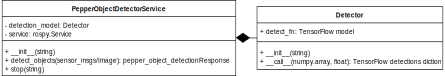
\includegraphics[width=\textwidth]{DetectorUml}
	\caption{Diagramma UML (semplificato) classe \texttt{PepperObjectDetectorService}}
	\label{fig:detector_uml}
\end{figure}

Nel costruttore della classe viene inizializzato il servizio ROS, al quale viene associato come handler il metodo \verb|detect_objects|, e viene inoltre creato un oggetto del tipo \verb|Detector|, che carica il modello di object detection dal percorso fornito e lo esegue sugli input che gli vengono sottomessi tramite chiamata. Il \verb|Detector| viene utilizzato in \verb|detect_objects| per eseguire la detection sugli input inviati al servizio.

Quando il nodo server viene eseguito, viene istanziato un oggetto del tipo 
\verb|PepperObjectDetectorService|, ed il suo metodo \verb|stop| viene registrato per l'esecuzione al momento dello shutdown del nodo, in modo tale che il servizio venga stoppato quando l'esecuzione del server termina. 
Infine il nodo entra in \verb|spin|, in modo da restare in ascolto delle richieste all'object detector.

\subsection{Server di interfaccia verso Pepper}

Il tale nodo è stato implementato per offrire le funzionalità offerte dal NAOqi Framework\footnote{Il framework usato per programmare i robot dell'\textbf{Aldebaran}, risponde alle più comuni esigenze della robotica.} senza obbligare il programmatore a scrivere codice \verb|python2|.

Come anticipato, si occupa di esporre tre servizi: text to speech, gestione della posa e movimento della testa di Pepper. 
Questi servizi sono stati implementati attraverso una classe chiamata \verb|NaoServer|, nel cui costruttore vengono inizializzati i tre servizi ROS e viene imposta al robot la lingua inglese.

Al servizio \verb|pepper_head_mover| è stato associato come handler il metodo \verb|moveHead|, che offre un interfaccia simile a quella del metodo \verb|angleInterpolation| del proxy NAOqi chiamato \verb|ALMotion|, al quale inoltrerà la richiesta di movimento. Di fatti, il metodo del proxy NAOqi offre anche la possibilità di effettuare movimenti rispetto ad indicazioni relative, non solo assolute.

Al servizio \verb|pepper_pose| è stato associato come handler il metodo \verb|setPose|, che offre un interfaccia simile a quella del metodo \verb|goToPosture| del proxy NAOqi chiamato \verb|ALRobotPosture|, al quale inoltrerà la richiesta di movimento. Di fatti, il metodo del proxy NAOqi offre anche la possibilità di effettuare il movimento a velocità diverse, nel nostro caso abbiamo ritenuto opportuno che il robot si muovesse al $10\%$ della sua velocità massima.

Al servizio \verb|pepper_tts| è stato associato come handler il metodo \verb|say|, che offre la medesima interfaccia del metodo \verb|say| del proxy NAOqi chiamato \verb|ALTextToSpeech|, al quale inoltrerà la sua richiesta.

I tre servizi, portato a termine il lavoro richiesto, invieranno al nodo che li invoca un valore booleano, indice del successo o insuccesso dell'operazione.

Quando il nodo server viene eseguito entra in \verb|spin|, in modo da restare in attesa di ricevere richieste.

\subsection{Nodo Master}

Il nodo Master (come \emph{puppet master}, ossia il burattinaio) è stato concepito come il pezzo centrale della nostra applicazione. Questo nodo si interfaccia con tutti i nodi dell'architettura, ed esegue i passi chiave del task in maniera sequenziale. La sequenza di passi è strettamente legata al task, e risulta molto semplice implementare un nuovo nodo che lo sostituisca per personalizzare o modificare i passi, compatibilmente con le interfacce che sono a disposizione nella nostra architettura.

Abbiamo scelto l'approccio sequenziale per semplicità di implementazione. Ciò non toglie che alcune delle azioni possano ottimizzate tramite parallelismi e sincronizzazioni, ma è stato scelto di posticipare questi miglioramenti per dare precedenza al funzionamento completo del sistema secondo le specifiche.

Qui presentiamo la sequenza di operazioni che compie il nodo.
% FRASE DI INIZIO DELLE FASI
\begin{enumerate}
	\item Aspetta che tutti i servizi siano online prima di poter proseguire.
	\item Porta il robot in una posizione neutra con il servizio \verb|pepper_pose| del nodo interfaccia. 
	\item Fa muovere la testa al robot in alcune posizioni predefinite, in cui verrà ``scattata'' una fotografia. Utilizza il servizio \verb|pepper_head_mover| per passare delle traiettorie con posizione singola, visto che dovrà aspettare una immagine dal topic della camera del robot. Nell'attuale implementazione, vengono assunte dieci posizioni che dividono la vista del robot in una matrice $5 \times 2$, in modo che le immagini risultanti siano leggermente sovrapposte.
	\item Esegue lo stitching delle immagini catturate con la libreria OpenCV, ottenendo così un'immagine panoramica di tutta la scena.
	\item Richiede al servizio \verb|pepper_object_detection| gli oggetti presenti nell'immagine panoramica.
	\item Genera una frase per il robot, dividendo gli oggetti trovati tra sinistra, centro e destra, che viene poi inviata al servizio \verb|pepper_tts| per essere riprodotta.
\end{enumerate}

\begin{figure}
	\centering
	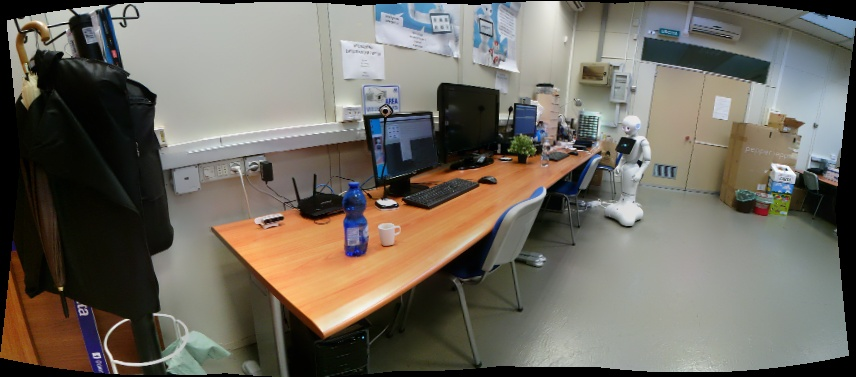
\includegraphics[width=\textwidth]{panorama}
	\caption{Vista del robot dopo l'image stitching.}\label{fig:panorama}
\end{figure}

Una scelta chiave che abbiamo preso è stata quella di eseguire uno stitching sulle immagini della vista (figura~\ref{fig:panorama}). I vantaggi di questo approccio sono molteplici: \begin{enumerate*}[label={(\arabic*)}] \item siamo in grado rilevare efficacemente oggetti che occupano uno spazio che vada oltre la singola immagine (es.\@: un tavolo); \item siamo in grado di evitare che oggetti piccoli divisi su più immagini vengano rilevati più volte, o nessuna; \item permette di allargare il campo visivo a piacere, aggiungendo più catture sia in orizzontale che in verticale.\end{enumerate*} Utilizzando altri approcci, alcune di queste proprietà sarebbero state sostanzialmente più complicate da implementare, e molto probabilmente non avrebbero avuto la stessa robustezza.

Avere una sola immagine fa sì che il detector lavori una sola volta. Se ciò sia effettivamente vantaggioso rispetto ad effettuare la detection su più immagini separate dipende da due fattori: il numero di immagini su cui fare la detection e il modello utilizzato. Nel caso di più immagini potrebbe bastare un detector leggero, visto che queste sono piccole e gli oggetti sono di meno e occupano gran parte della scena. Nel nostro caso, invece, l'immagine risulterà più grande, e soprattutto conterrà più oggetti che occuperanno, relativamente alle dimensioni, meno spazio. Come vedremo nel prossimo paragrafo, sarà necessaria una rete più precisa nel localizzare oggetti piccoli, e quindi più complessa.
\section{Detector}

\begin{comment}
    Breve descrizione e motivazione della scelta
    Tabellina che abbiamo fatto noi
    Tabellina di Object Recognition Model Zoo
    Almeno immagine finale
\end{comment}


Nello scegliere il modello abbiamo considerato come use-case di riferimento il task assegnatoci per l'esercitazione, senza calarci in una situazione di utilizzo del robot specifica (ad esempio assistenza domiciliare). Pertanto, abbiamo ritenuto necessario dare più importanza alla precisione del risultato che ai tempi di esecuzione. In un'eventuale interazione con un utente, infatti, degli errori di detection più grossolani risalterebbero maggiormente rispetto ad un tempo di attesa prolungato. Ovviamente anche quest'ultimo ha la sua importanza, visto che non ricevere feedback per un determinato lasso di tempo potrebbe suscitare preoccupazione nell'utente. Sull'hardware fornito per il progetto ci è impossibile tener conto del tempo di esecuzione, che risulta eccessivo con la maggior parte delle reti, anche quelle poco performanti. Ciò considerato, la scelta che abbiamo fatto minimizza i tempi di esecuzione tenendo però conto della precisione necessaria affinché l'interazione risulti soddisfacente.
In particolare, rispetto a quest’ultimo aspetto non ci è possibile fornire una valutazione quantitativa delle performance, in quanto davanti al robot si presenta sempre la stessa scena, pertanto abbiamo valutato i detector in base al loro comportamento relativamente a questa scena, e quindi i giudizi nella colonna “Performance” della tabella~\ref{table:modelli} fanno riferimento soltanto a questa condizione. Inoltre, le immagini che abbiamo catturato, a valle dello stitching, hanno una dimensione di circa $900 \times 400$. Durante le nostre prove ci siamo accorti che questo tipo di immagini non sono tipici input per le reti a nostra disposizione. Infatti alcune di queste, nonostante avessero valori di mAP di tutto rispetto sul dataset COCO\footnote{\url{https://github.com/tensorflow/models/blob/master/research/object_detection/g3doc/tf2_detection_zoo.md}}, non risultavano efficaci nella situazione in esame.



Inizialmente sono state provate due reti che lavorano con immagini aventi risoluzione $640 \times 640$ che, però, facendo un downscale dell’immagine risultato del processo di stitching, hanno dimostrato pessime performance.
Abbiamo quindi deciso di provare reti che lavorano con immagini aventi una risoluzione più grande. La Faster-RCNN che usa come backbone ResNet101 con input size $1024 \times 1204$, avendo performance discrete nella detection (non tutti gli oggetti venivano rivelati ed ad altri veniva assegnata l’etichetta sbagliata), ha dimostrato che la risoluzione delle immagini in input deve essere un altro fattore discriminante nella scelta del modello.

Il passo successivo è stato provare una rete che lavorasse con immagini più simili, in risoluzione, a quelle che noi le forniamo in input: Faster-RCNN con backbone ResNet50 ha dimostrato, in tempi simili alle altre reti, ottime performance in termini di rilevazione degli oggetti, ma a qualche oggetto veniva assegnata una label sbagliata; Faster-RCNN con backbone ResNet101 ha dimostrato le migliori performance sia per la classificazione che per la detection, ma in tempi più dilatati, pertanto abbiamo preferito tenere come nostro modello di riferimento Faster-RCNN basata su ResNet50. I dati sui confronti tra questi modelli sono riportati in tabella~\ref{table:modelli}.

\begin{table}
    \centering
    \begin{tabular}{|c|c|c|c|} 
     \hline
     \textbf{Modello} & \textbf{Input size} & \textbf{Tempo} & \textbf{Prestazioni} \\
     \hline
     SSD MobileNetV1 & $640 \times 640$ & $6$ sec & Scarse \\
     \hline
     SSD ResNet152 V1 FPN & $640 \times 640$ & $20$ sec & Molto scarse \\
     \hline
     EfficientDet D3 & $896 \times 896$ & $23$ sec & Buone \\
     \hline
     Faster-RCNN ResNet101 & $1024 \times 1024$ & $20$ sec & Buone \\
     \hline
     Faster-RCNN ResNet50 & $800 \times 1333$ & $21$ sec & Ottime \\
     \hline
     Faster-RCNN ResNet101 & $800 \times 1333$ & $30$ sec & Migliori \\
     \hline
    \end{tabular}
    \caption{Confrontro tra i modelli testati. La input size è fornita in formato $h\times w$, mentre il tempo è relativo all'inferenza su una singola immagine, eseguita su una CPU virtualizzata.}
    \label{table:modelli}
\end{table}

Questo modello consiste di una \emph{Region Proposal Network} (RPN) e una rete che si occupa della classificazione, ed entrambe condividono le feature convoluzionali dell'intera immagine. Pertanto, le feature maps estratte dai layer convoluzionali sono date in input alla RPN, la quale utilizza una sliding window sulle feature maps, e per ogni finestra genera $k$ anchor boxes di diverse forme e grandezze aventi centro coincidente con quello della finestra \cite{resnet}\todo{aggiungere info sulla parte restante della rete, prendendo come backbone ResNet50}. In letteratura è riscontrabile come Faster-RCNN sia una delle architetture migliori per le detection su oggetti di medie e piccole dimensioni, principalmente presenti nelle nostre immagini (vedi paragrafo~\ref{sec:master_small_img}).

\begin{figure}
    \centering
    \hfill
    \begin{subfigure}[b]{0.49\textwidth}
        \centering
        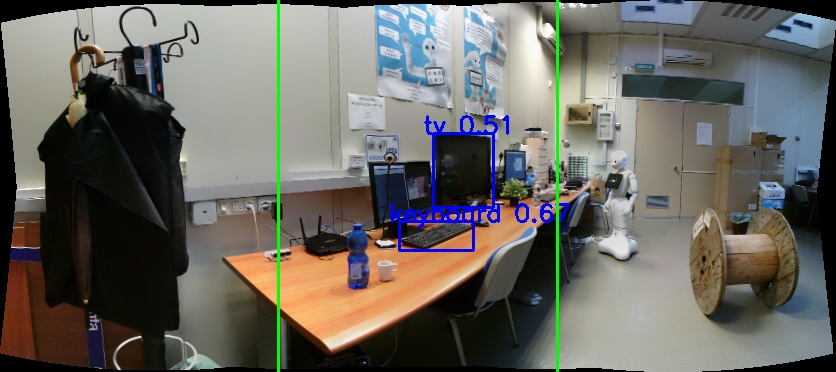
\includegraphics[width=\textwidth]{ssd_mobilenet}
        \caption{SSD MobileNetV1}
    \end{subfigure}
    \hfill
    \begin{subfigure}[b]{0.49\textwidth}
        \centering
        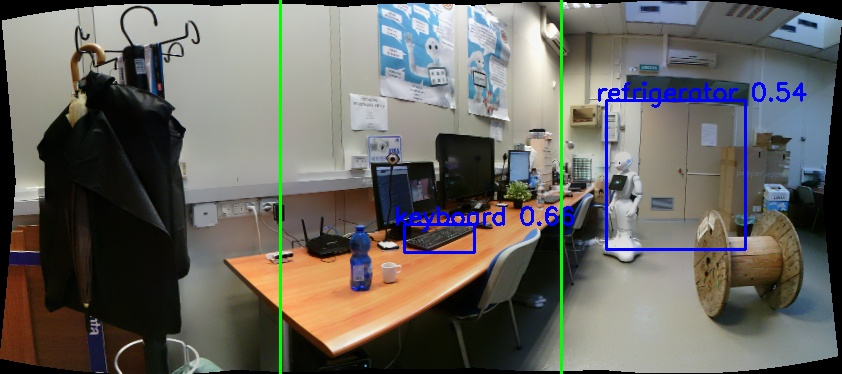
\includegraphics[width=\textwidth]{ssd_resnet152}
        \caption{SSD ResNet101}
    \end{subfigure}
    \hfill \\
    \hfill
    \begin{subfigure}[b]{0.49\textwidth}
        \centering
        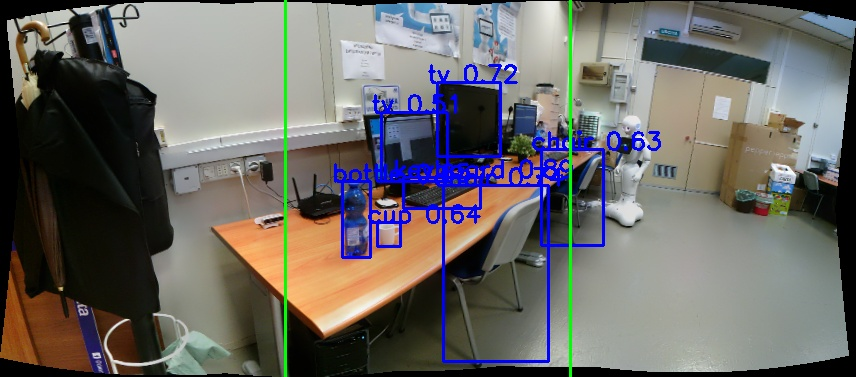
\includegraphics[width=\textwidth]{efficientdetd3}
        \caption{EfficientDet D3}
    \end{subfigure}
    \hfill
    \begin{subfigure}[b]{0.49\textwidth}
        \centering
        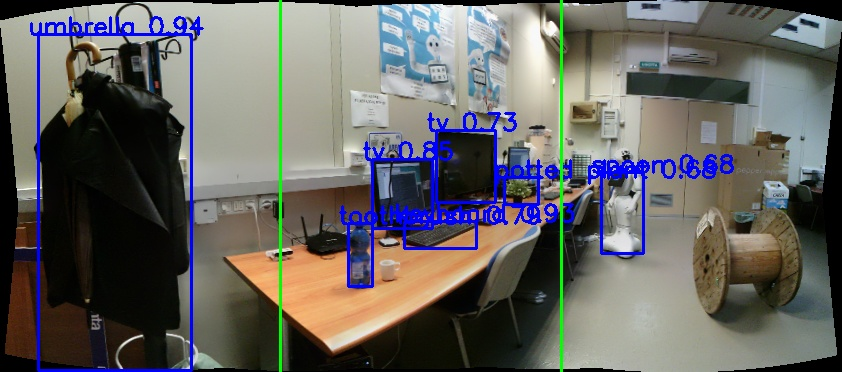
\includegraphics[width=\textwidth]{fastercnnresnet101-1024x1024.jpg}
        \caption{Faster-RCNN ResNet101 $1024\times 1024$}
    \end{subfigure}
    \hfill \\
    \hfill
    \begin{subfigure}[b]{0.49\textwidth}
        \centering
        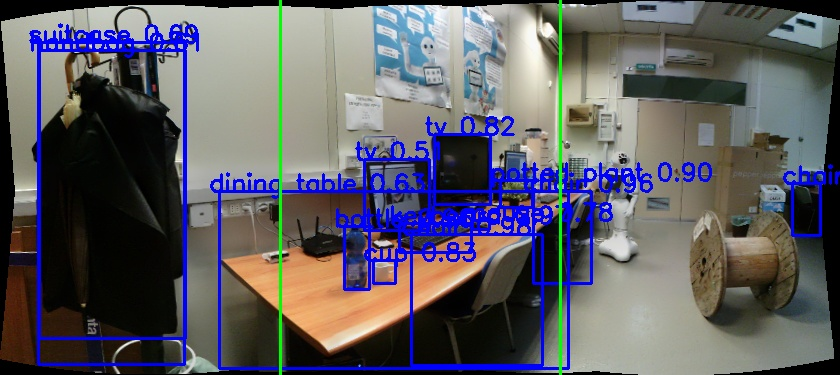
\includegraphics[width=\textwidth]{fastercnnresnet50-800x1333.jpg}
        \caption{Faster-RCNN ResNet50 $800\times 1333$}
    \end{subfigure}
    \hfill
    \begin{subfigure}[b]{0.49\textwidth}
        \centering
        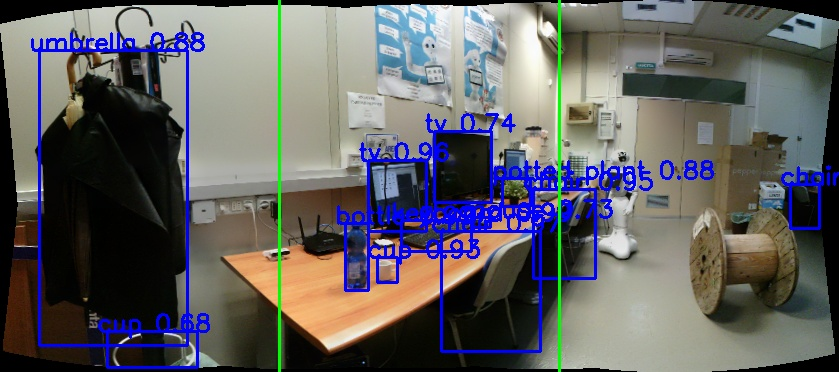
\includegraphics[width=\textwidth]{fastercnnresnet101-800x1333.jpg}
        \caption{Faster-RCNN ResNet101 $800\times 1333$}
    \end{subfigure}
    \hfill
    \caption{Risultati dei modelli testati. Le bande verticali di colore verde fluo evidenziano la suddivisione dell’immagine utilizzata per separare tra loro le regioni sinistra, destra e centrale.}
\end{figure}
\section{Conclusioni}

Come possibili sviluppi futuri del progetto proponiamo: \todo{CHECK aggiunti gli articoli ai punti della lista}
\begin{itemize}
    \item l'utilizzo di una tecnica diversa dall'image stitching per evitare rilevazioni ripetute degli stessi oggetti in frame diversi;
    \item la re-implementazione sotto forma di azioni ROS delle diverse funzionalità che attualmente sono realizzate come servizi ROS, in modo da poter, ad esempio, avviare la detection quando Pepper inizia a riportare la testa nella posizione iniziale, ed eseguire le due operazioni contemporaneamente, così da ottimizzare il tempo totale di interazione;
    \item l'esecuzione del software utilizzando dispositivi di accelerazione per reti neurali, sia a bordo di Pepper, ad esempio utilizzando una delle schede Nvidia Jetson, che a distanza, ad esempio usando una GPU su di un server dedicato, al fine di misurarne le reali prestazioni in termini di tempo di esecuzione;
    \item una valutazione delle performance in termini di rilevamento e classificazione su scene diverse.
\end{itemize} 

%\section{Descrizione della soluzione}
%\subsection{Architettura}

\begin{figure}[ht]
	\centering
	\includegraphics[width=\textwidth]{Architettura}
	\caption{Architettura del software}
	\label{fig:architecture}
\end{figure}

Il nostro software si compone di tre nodi:
Un nodo che implementa il servizio di object detection, che riceve in input un’immagine da analizzare e, per ogni oggetto nell’immagine, restituisce il relativo bounding box, la classe ed il livello di confidenza relativo alla predizione.
Un nodo che implementa tre servizi che forniscono un’interfaccia verso le funzionalità di text to speech, gestione della posa e movimento della testa di Pepper.
Un nodo master che implementa la funzionalità richiesta dall’homework acquisendo le immagini dal topic della camera di Pepper e utilizzando i servizi offerti dagli altri due nodi.
Per l’interfacciamento da e verso Pepper viene utilizzato il NaoQi SDK.

\subsection{Choices}

BULLET 1
Abbiamo implementato le interfacce verso le funzionalità del robot (TTS, movimento della testa e gestione della posa) come servizi perché questo permette di modellare queste funzionalità come risorse condivise tra i vari nodi e di gestire gli accessi ad esse. L'utilizzo del paradigma request-response al posto di quello publish-subscribe permette inoltre di attendere e verificare l'esito di un'operazione, cosa molto utile quando si lavora con sistemi fisici.
Non abbiamo utilizzato un'azione (non bloccante) perché per la nostra applicazione era comodo bloccare il sistema in attesa del completamento delle operazioni sul robot.

Per quanto riguarda le funzionalità di object detection, anch'esse sono fornite tramite un servizio, perché così facendo non è necessario inserire nel messaggio che trasporta il risultato della detection l'immagine di riferimento, in quanto il nodo che effettua la richiesta al servizio sa quale immagine sta fornendo in input, permettendo così di mantenere il messaggio più snello e di semplificare la sincronizzazione tra nodi che richiedono un'operazione di detection ed il nodo che la realizza.
Abbiamo scelto un servizio e non un'azione perché per la nostra applicazione non è necessario fare altro mentre è in corso una detection.
Come nota a margine, si fa notare che il fatto che il detector restituisca il risultato al solo nodo che invia la richiesta potrebbe sembrare limitante nel caso in cui il risultato della detection su di una stessa immagine dovesse servire per più nodi, perché si potrebbe pensare di dover invocare più volte il servizio fornendo la stessa immagine in input. In realtà, questa cosa può essere evitata facendo in modo che un solo nodo invochi il servizio e pubblichi il risultato ottenuto su di un apposito topic. Questo sistema, rispetto all'utilizzo del paradigma publish-subscribe, consente di conservare la possibilità di ricevere un feedback sul risultato dell'operazione. 

BULLET 2
Per gestire i parametri di configurazione utilizziamo il parameter server di ROS e un file di configurazione che viene automaticamente caricato su di esso tramite il nostro launch file.

BULLET 3
Per il task di visione abbiamo scelto di catturare più immagini della scena e di farne lo stitching. In tutto catturiamo 10 immagini, ruotando la testa tra 0.8 e -0.8 rad lungo l'asse z (yaw), e tra 0.2 e -0.2 rad lungo l'asse y (pitch). 

Fare l'image stitching ha i seguenti vantaggi:
* Permette di vedere oggetti grandi che occupano più spazio di una sola immagine
* Permette di evitare che oggetti piccoli divisi su due immagini possano essere visti due volte o nessuna
* Permette di allargare il campo visivo sia in orizzontale che in verticale, scegliendo opportunamente il numero e la posizione delle catture.

Avere una sola immagine fa sì che il detector lavori una sola volta. Se ciò sia effettivamente vantaggioso rispetto ad effettuare la detection su più immagini separate dipende da due fattori: il numero di immagini su cui fare la detection e il modello utilizzato. Nel caso di più immagini potrebbe bastare un detector leggero, visto che queste sono piccole e gli oggetti sono di meno e occupano gran parte della scena. Nel nostro caso, invece, l'immagine risulterà più grande, e soprattutto conterrà più oggetti che occuperanno, relativamente alle dimensioni, meno spazio. Come vedremo nella prossima slide, ci sarà bisogno di un detector più complesso.




%\section{Risultati sperimentali}
%\subsection{Models comparison}

La scelta del modello è stata dettata da tre parametri: la risoluzione delle immagini in ingresso, i tempi di esecuzione del detector per immagine e, infine, la sua capacità di individuare e classificare correttamente gli oggetti. In particolare, rispetto a quest’ultimo aspetto non ci è possibile fornire una valutazione quantitativa delle performance, in quanto davanti al robot si presenta sempre la stessa scena, pertanto abbiamo valutato i detector in base al loro comportamento relativamente a questa scena, e quindi i giudizi nella colonna “Performance” della tabella fanno riferimento a questa condizione. Inoltre, le immagini che abbiamo catturato, a valle dello stitching, hanno una dimensione di circa 900x400. Durante le nostre prove ci siamo accorti che questo tipo di immagini non sono tipici input per le reti a nostra disposizione. Alcune di queste, nonostante avessero valori di mAP di tutto rispetto sul dataset COCO (come si può vedere su \url{https://github.com/tensorflow/models/blob/master/research/object_detection/g3doc/tf2_detection_zoo.md)}, non risultavano efficaci nella situazione in esame.

Inizialmente sono state provate due reti che lavorano con immagini aventi risoluzione 640x640, tali detector, facendo un downscale dell’immagine risultato del processo di stitching, hanno dimostrato pessime performance.
Abbiamo quindi deciso di provare reti che lavorano con immagini aventi una risoluzione più grande. La Faster RCNN che usa come backbone Resnet 101 e che lavora con immagini aventi una risoluzione di 1024x1204, avendo performance discrete nella detection (non tutti gli oggetti venivano rivelati ed ad altri veniva assegnata l’etichetta sbagliata), ha dimostrato che la risoluzione delle immagini date in input ai modelli deve essere un fattore discriminante nella scelta del modello.
Il passo successivo è stato, quindi, quello di provare una rete che lavorasse con immagini più simili, in risoluzione, a quelle che noi le diamo in input: la Faster RCNN che usa come backbone Resnet 50, ha dimostrato, in tempi ragionevoli, ottime performance in termini di rilevazione degli oggetti, ma a qualche oggetto veniva assegnata una label sbagliata; la Faster RCNN che usa come backbone Resnet 101 ha dimostrato le migliori performance sia per la classificazione che la detection, ma in tempi meno ragionevoli.

Nelle immagini riportanti i risultati delle detection con le varie reti, le bande verticali di colore verde fluo evidenziano la suddivisione dell’immagine utilizzata per separare tra loro le regioni sinistra, destra e centrale.

I tempi di esecuzione riportati nella tabella fanno riferimento all’esecuzione della rete all’interno della VM “di riferimento” per il corso, senza l’utilizzo di accelerazione basata su GPU. Inoltre, sono tempi “di regime”, cioè validi per tutte le esecuzioni del detector eccetto la prima, che, sperimentalmente, per motivi probabilmente legati a TensorFlow, impiega considerevolmente più tempo delle altre.

\subsection{The chosen model}

Si può notare come lo stitching permetta di fornire in input al detector una visione d’insieme della scena, che consente ad esempio di rilevare oggetti quali la scrivania, che sarebbero stati più difficili da individuare attraverso l’analisi di singole catture successive.


\printbibliography
\end{document}
